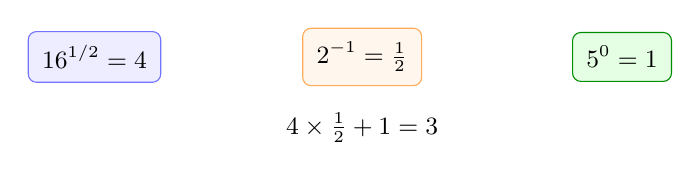
\begin{tikzpicture}[font=\small]
        \node[draw=blue!55,fill=blue!7,rounded corners=3pt,inner sep=5pt] at (0,0) {$16^{1/2}=4$};
        \node[draw=orange!65,fill=orange!7,rounded corners=3pt,inner sep=5pt] at (3.4,0) {$2^{-1}=\frac12$};
        \node[draw=green!55!black,fill=green!10,rounded corners=3pt,inner sep=5pt] at (6.7,0) {$5^0=1$};
        \node at (3.4,-0.9) {$4\times\frac12+1=3$};
    \end{tikzpicture}
